% !TEX program = xelatex
\documentclass{article}
\usepackage{xcolor} % 在latex中使用颜色
\usepackage{booktabs,tabularx,multicol} % 制作表格
\usepackage{framed} % 制作文本框
\usepackage{amsmath,amsthm,amssymb,amsfonts}    % 数学符号与字体
\usepackage{hyperref}   % 添加超链接
\usepackage[left=2.0cm, right=2.0cm, top=2.5cm, bottom=2.5cm]{geometry} % 调整页边距
\usepackage{appendix}   % 附录环境
\usepackage{subfig,graphicx}    % 插入照片

%---------------优雅的插入MATLAB代码---------%
\usepackage{listings,matlab-prettifier} % MATLAB 美化包
\lstset{
        style=Matlab-editor,
        basicstyle=\mlttfamily,
        escapechar=`,
        numbers      = left,
        numbersep    = 5pt,
        numberstyle  = \small\color{red},
        frame        = single,
        keepspaces   = true,
        tabsize      = 4,
        breaklines = true,
}
%-------------标题-------------%
\author{}
\date{\today}
\title{}

%-----------做一些设置-----------%
\numberwithin{equation}{section}    % 公式标号与section的编号挂钩

%------------自定义一些命令------------%
\newcommand{\upcite}[1]{\textsuperscript{\textsuperscript{\cite{#1}}}}
\newcommand*{\dif}{\mathop{}\!\mathrm{d}}
\def\degree{${}^{\circ}$}

%---------配置环境------------%
\definecolor{shadecolor}{RGB}{241,241,255}
\newcounter{problemname}
\newenvironment{problem}{\begin{shaded}\stepcounter{problemname}\par\noindent\textbf{题目\arabic{problemname}. }}{\end{shaded}\par}
\newenvironment{solution}{\par\noindent\textbf{解答. }}{\par}
\newenvironment{note}{\par\noindent\textbf{题目\arabic{problemname}的注记. }}{\par}

%-------------可控列宽的表格--------%
\newcolumntype{R}[1]{>{\raggedright\arraybackslash}p{#1}}
\newcolumntype{C}[1]{>{\centering\arraybackslash}p{#1}}
\newcolumntype{L}[1]{>{\raggedleft\arraybackslash}p{#1}}


\begin{document}

\section{(a)}
\lstinputlisting[caption={\bf sol\_tri\_matrix.m}]{code/sol_tri_matrix.m}
\section{(b)}
\lstinputlisting[caption={\bf get\_coefficients.m}]{code/get_coefficients.m}
\section{(c)}
\lstinputlisting[caption={\bf get\_yy.m}]{code/get_yy.m}
\section{(d)}
\lstinputlisting[caption={\bf main.m}]{code/main.m}




\begin{figure}[htbp]%
    \centering
    \subfloat[$n=16$]{
        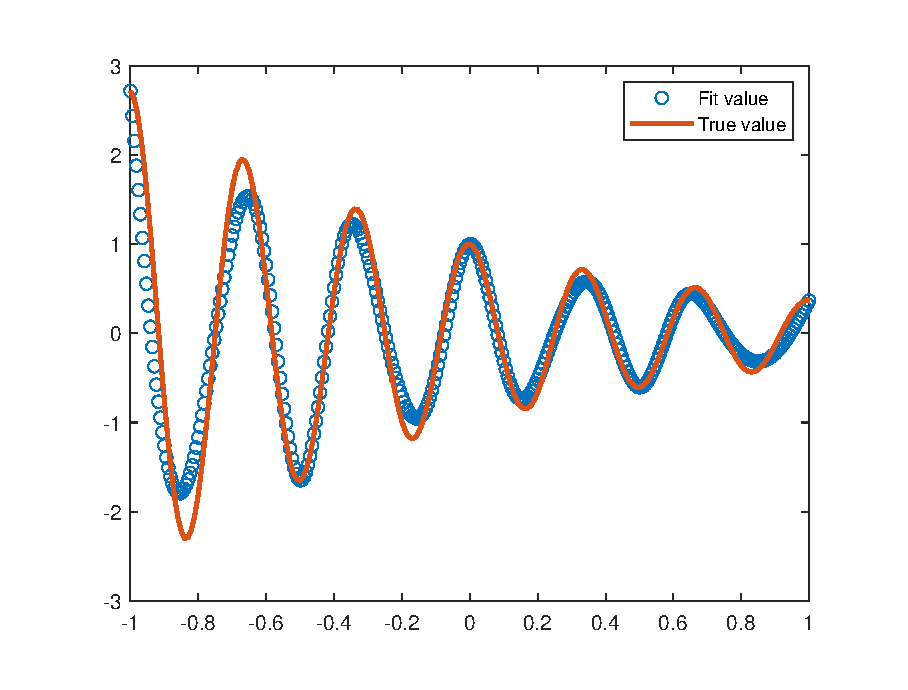
\includegraphics[width=0.45\linewidth]{fig/pic1.eps}
        }\hfill
    \subfloat[$n=32$]{
        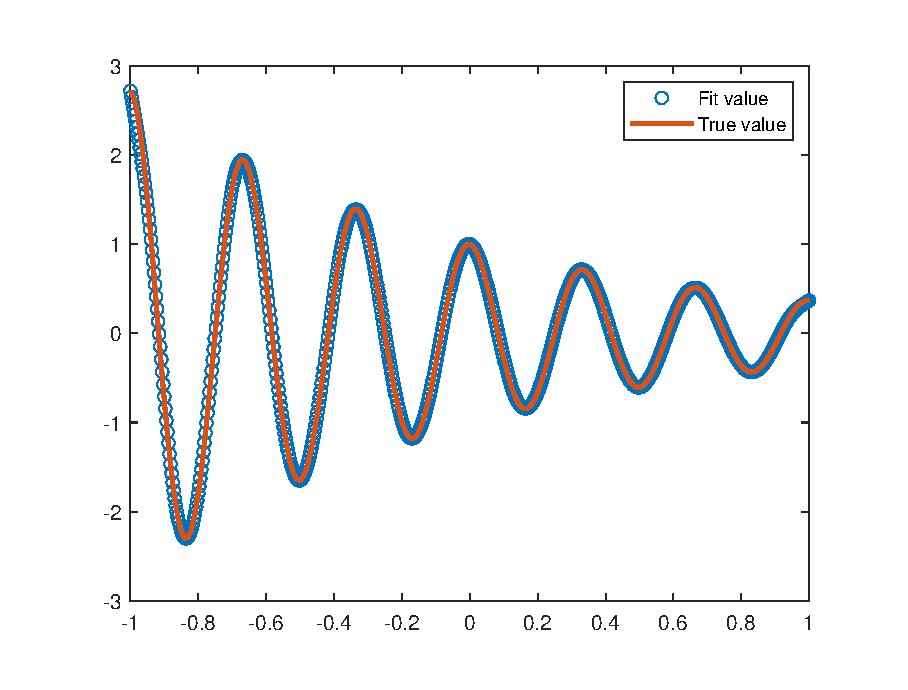
\includegraphics[width=0.45\linewidth]{fig/pic2.eps}
        }\\
    \subfloat[$n=64$]{
        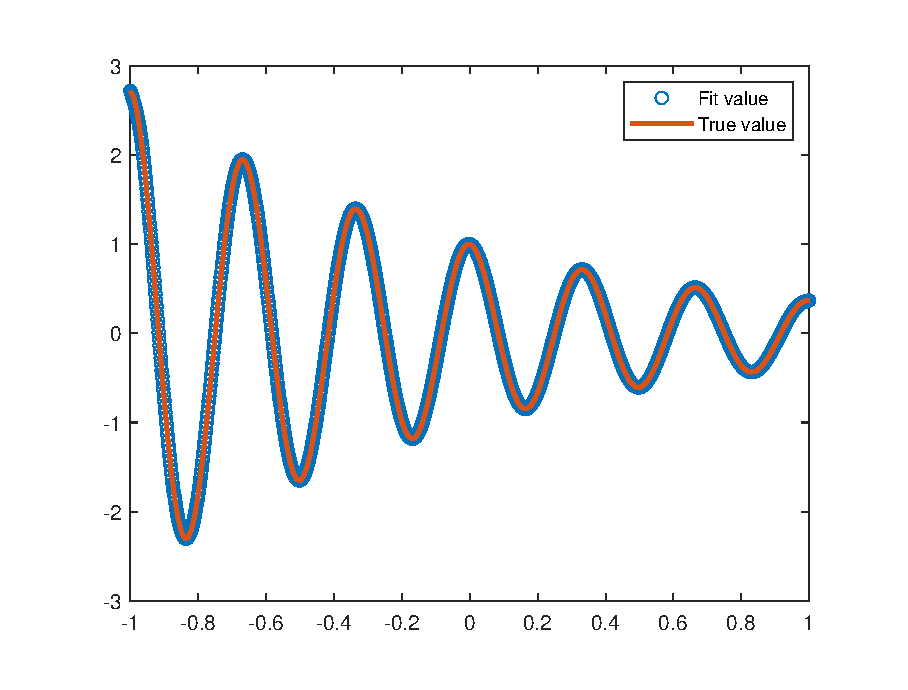
\includegraphics[width=0.45\linewidth]{fig/pic3.eps}
        }\hfill
    \subfloat[$n=128$]{
        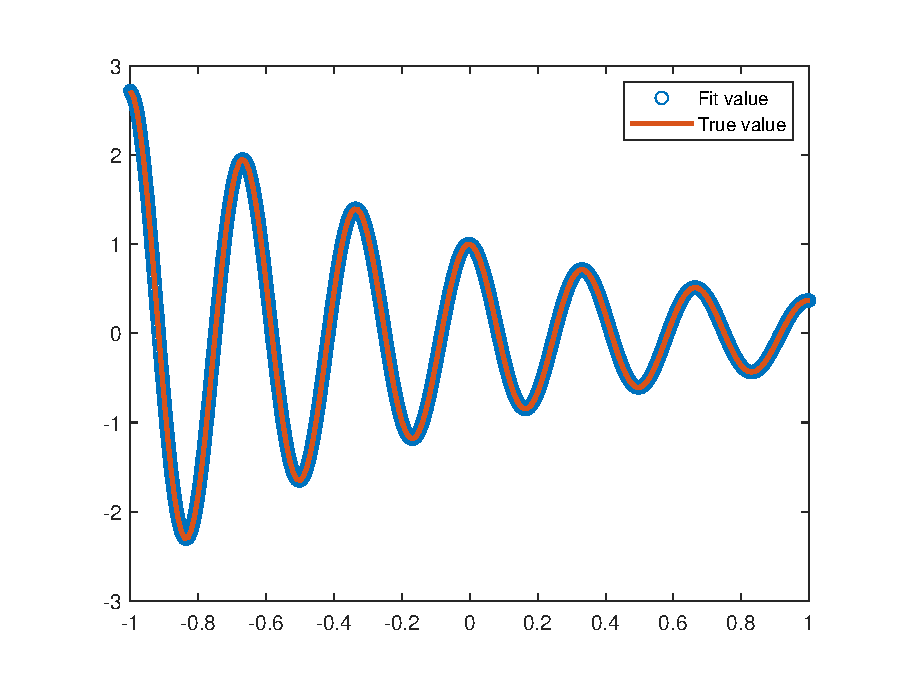
\includegraphics[width=0.45\linewidth]{fig/pic4.eps}
        }\\    
    \caption{The fitting effect varies with n}
    \label{4figs}
\end{figure}
\begin{figure}[htp]
    \centering
    \includegraphics[width=0.45\linewidth]{fig/pic5.eps}
    \caption{Error analysis}

\end{figure}
\clearpage
The magnitude of the error E of the solution for the maximum error for different n values is shown. In the log-log plot, the error is a function of n, which is essentially a straight line with a slope of -2, meaning that $lg E approx alpha + blg n$, where $b=-2$; in other words, the error is $Eapprox Kn^{-2}$

\end{document}